\subsection{Big Data Projects}

\begin{remark} \hlt{ML Model Building Steps for Structured Data}
\begin{enumerate}[label=\roman*.]
\setlength{\itemsep}{0pt}
\item Conceptualisation of modelling task: define output, user, usage in existing or new processes
\item Data collection: whether from internal or external source
\item Data preparation and wrangling: cleansing, pre-processing of data
\item Data exploration: Exploratory Data Analysis (EDA), feature selection, feature engineering
\item Model training: select ML method, evaluate performance, tuning model
\end{enumerate}
\end{remark}

\begin{remark} \hlt{ML Model Building Steps for Unstructured Data}
\begin{enumerate}[label=\roman*.]
\setlength{\itemsep}{0pt}
\item Problem formulation: define input and output, usage, purpose
\item Data curation: via web scraping, and annotation of labels.
\item Text preparation and wrangling: convert data to usable format
\item Text exploration: create word clouds, text feature selection and engineering
\end{enumerate}
\end{remark}

\begin{figure}[H]
\centering
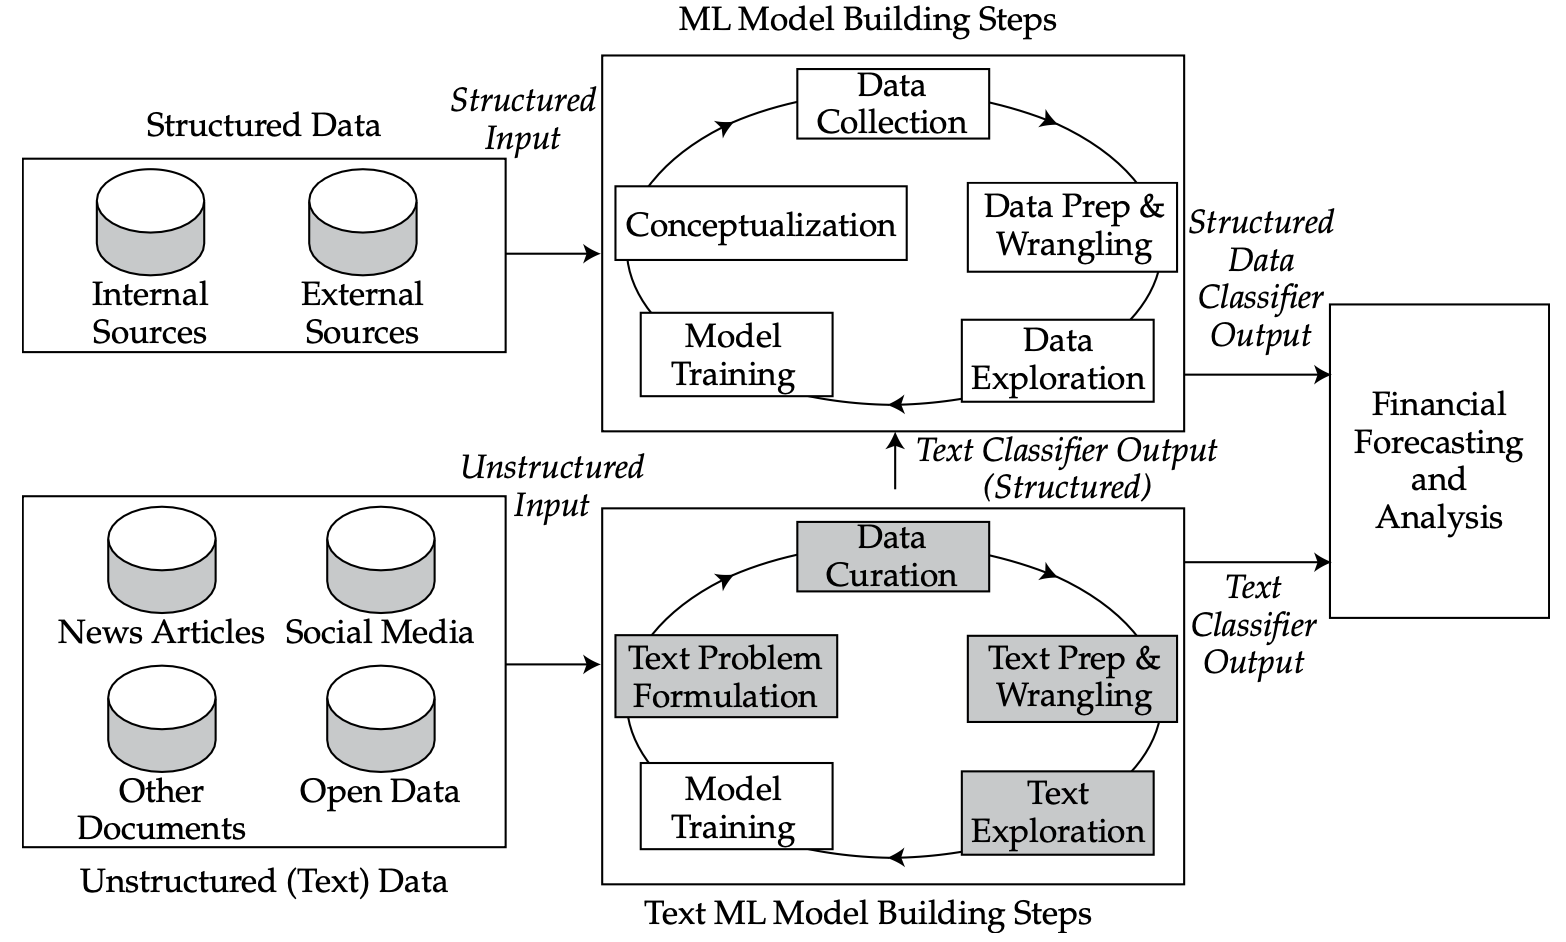
\includegraphics[scale=0.45]{/quant/mlbuild}
\caption{Model building for financial forecasting using big data}
\end{figure}

\begin{definition} \hlt{Data Cleansing}\\
Deals with reducing errors in raw data. Spot incomplete, duplicated, erroneous, or inaccurate values.\\
Metadata (summary data) may serve as starting point for error identification
\end{definition}

\begin{definition} \hlt{Data Wrangling}\\
Preprocessing the data for model use. Includes dealing with outliers, extract useful variables from existing data points, scaling the data, feature selection, aggregation of variables.
\end{definition}

\begin{definition} \hlt{Types of Data Errors and Rectification}
\begin{enumerate}[label=\roman*.]
\setlength{\itemsep}{0pt}
\item Incompleteness error: missing values and NA to be omitted or substituted
\item Invalidity error: data outside of meaningful range. Data to be verified.
\item Inaccuracy error: data not a measure of true value. To be rectified with business records.
\item Inconsistency error: in conflict with rest of data. To clarify with another source.
\item Non-uniformity error: data not in same format. To be converted to same format.
\item Duplication error: to remove duplicate entries.
\end{enumerate}
\end{definition}

\begin{remark} \hlt{Dealing with Outlier Data}
\begin{enumerate}[label=\roman*.]
\setlength{\itemsep}{0pt}
\item Trimming: removing highest and lowest $\alpha \%$ of observations
\item Winsorisation: extreme values replaced by maximum value allowable for that variable
\end{enumerate}
\end{remark}

\begin{remark} \hlt{Conversion of Data Features}
\begin{enumerate}[label=\roman*.]
\setlength{\itemsep}{0pt}
\item Normalisation: scales values between $0$ and $1$.
\begin{equation}
X_i = \frac{X_i - X_{\min}}{X_{\max} - X_{\min}} \nonumber
\end{equation}
\item Standardisation: centres variables at $0$, then scales them as standard deviations from mean.
\begin{equation}
X_i = \frac{X_i - \mu}{\sigma} \nonumber
\end{equation}
\end{enumerate}
Normalisation is sensitive to outliers. Standardisation is less sensitive to outliers
\end{remark}

\begin{method} \hlt{Text Preparation or Cleansing}
\begin{enumerate}[label=\roman*.]
\setlength{\itemsep}{0pt}
\item Remove HTML text using regular expression (regex).
\item Remove punctuations, except percentage, currency symbols, question marks. These to be substituted with annotations to preserve grammatical meaning.
\item Remove numbers and substituted with annotation /number/, except if of interest
\item Remove white spaces
\end{enumerate}
\end{method}

\begin{method} \hlt{Text Tokenisation (Normalisation of Text)}
\begin{enumerate}[label=\roman*.]
\setlength{\itemsep}{0pt}
\item Lowercase all alphabets to remove distinction among the same words
\item Stop words removed to reduce number of tokens in training set, except if critical
\item Stemming: convert inflicted forms of word to its base word. Porter’s algorithm may be used.
\item Lemmatisation: convert inflicted forms of word into its morphological root.
\end{enumerate}
Stemming, lemmatisation reduce repetition of words in various forms.
\end{method}

\begin{remark} \hlt{Output of Text Tokenisation}
\begin{enumerate}[label=\roman*.]
\setlength{\itemsep}{0pt}
\item Bag of words (BOW): collection of distinct set of tokens from all text in sample data
\item Document term matrix (DTM): each row is a document, each column is a token. 
\item N-grams: representation of word sequences. Provide context for advanced ML.
\end{enumerate}
\end{remark}

\begin{method} \hlt{Exploratory Data Analysis (EDA)}\\
Uses visualisation to summarise and observe data. To understand data properties, find patterns and relationships in data, inspect basic questions and hypothesis, document data distribution and characteristics, plan modelling strategies for next steps.
\begin{enumerate}[label=\roman*.]
\setlength{\itemsep}{0pt}
\item Feature selection: only pertinent features selected for training. Statistical measures used to assign a score gauging importance of each feature, then ranked.
\item Feature engineering: create new features by changing, transforming existing features
\item One-hot encoding: convert categorical variables into binary form.
\end{enumerate}
\end{method}

\begin{remark} \hlt{Text Exploration}
\begin{enumerate}[label=\roman*.]
\setlength{\itemsep}{0pt}
\item Term frequency (TF): ratio of number of times token occur, divided by total number of tokens.\\
To prune words with very low and very high TF values so as to remove noise.
\item Document frequency (DF): number of documents that contain token, divide by total document number.
\item Inverse document frequency (IDF): $IDF = \log (1/DF)$, measure how unique a term is.
\item TF-IDF: $=TF \times IDF$. A higher value means more frequent in smaller number of docs, hence indicates a more important word.
TF-IDF value varies by number of documents in dataset, hence performance vary if document number is small. Metric is calculated at the sentence level, not at collection level.
\item Word cloud: visualises the most informative words based on their TF value.
\end{enumerate}
\end{remark}

\begin{remark} \hlt{Feature Selection for Text}
\begin{enumerate}[label=\roman*.]
\setlength{\itemsep}{0pt}
\item Frequency measure used for vocabulary pruning, filter very high and low TF values.
\item $\chi^2$ test applied to test independence of $2$ events: occurrence of token and occur of class.\\
Test ranks tokens by usefulness to each class in text class probability.\\
Tokens with highest $\chi^2$-statistics occur more frequently in texts associated with a class, hence may be used as feature due to higher discriminatory potential.
\item Mutual information (MI) measures how much info is contributed by token to class of text.\\
$MI = 0$ if token distribution in all text class is same.\\
$MI = 1$ if token in any one class tends to occur more often in only that particular class of text.
\end{enumerate}
\end{remark}

\begin{remark} \hlt{Feature Engineering for Text}
\begin{enumerate}[label=\roman*.]
\setlength{\itemsep}{0pt}
\item Numbers: converted to token such as /number/
\item N-grams: multi-word patters that are discriminative identified, with connection intact
\item Name entity recognition (NER): analyse individual token and their surrounding semantics while referring to its dict to tag an object class to the token.\\
Can identify critical tokens on which lowercasing, stemming can be avoided.
\item Parts of speech (POS): tags words as noun, verb, adjective etc.\\
Useful for separating verbs and nouns for text analytics.
\end{enumerate}
\end{remark}

\begin{remark} \hlt{Causes of Model Fitting Errors}
\begin{enumerate}[label=\roman*.]
\setlength{\itemsep}{0pt}
\item Dataset size: small datasets lead to under-fitting the model
\item Number of features: may lead to under-fit or overfit.
\end{enumerate}
\end{remark}

\begin{remark} \hlt{Model Selection Factors}
\begin{enumerate}[label=\roman*.]
\setlength{\itemsep}{0pt}
\item Supervised or unsupervised learning: whether data is labelled/unlabelled, purpose of model
\item Type of data: numeric data use CART, text data use GLM and SVM. Image data use NN ad deep learning. Speech data use deep learning methods.
\item Size of data: type of models used depends on number of features and number of instances of data
\end{enumerate}
\end{remark}

\begin{definition} \hlt{Class Imbalance}\\
Number of instances for one class significantly larger than other classes. Not ideal for supervised learning.\\
Choice of under-sample or oversample depends on context.\\
Advanced techniques may reproduce synthetic data from existing data.
\end{definition}

\begin{flushleft}
Confusion Matrix\\
\begin{tabular}{|c|c|c|}
\hline
\rowcolor{gray!30}
Prediction vs Actual & Class $1$ & Class $0$ \\
\hline
Class $1$ & True Positives (TP) & False Positives (FP), Type I Error\\
\hline
Class $0$ & False Negatives (FN), Type II Error & True Negatives (TN)\\
\hline
\end{tabular}
\end{flushleft}

\begin{definition} \hlt{Model Performance Metrics}
\begin{enumerate}[label=\roman*.]
\setlength{\itemsep}{0pt}
\item Precision: ratio of true positives to all predicted positives.\\
High precision valued when cost of Type I error is large.
\begin{equation}
P = \frac{TP}{TP + FP} \nonumber
\end{equation}
\item Recall: ratio of true positives to all actual positives.\\
High recall valued when cost of Type II error is large.
\begin{equation}
R = \frac{TP}{TP + FN} \nonumber
\end{equation}
\item Accuracy: proportion of correct forecasts out of a total number of forecasts
\begin{equation}
\text{Accuracy} = \frac{TP + TN}{TP + FP + TN + FN} \nonumber
\end{equation}
\item $F1$ Score: harmonic mean of precision and recall.\\
More appropriate to be used when unequal class distribution is present in the dataset.
\begin{equation}
F1 \text{ Score} = \frac{2 \times P \times R}{P + R} \nonumber
\end{equation}
\end{enumerate}
\end{definition}

\begin{definition} \hlt{Receiver Operating Characteristic (ROC)}\\
Plots curve showing trade-off between false positive rate ($x$-axis) and true positive rate ($y$-axis).\\
More convex curve indicates better performance.\\
Area under the curve (AUC): $AUC \rightarrow 1$ is perfect prediction. $AUC \rightarrow 0.5$ is as good as random guess.
\begin{align}
TPR &= \frac{TP}{TP + FN}, \ \ \ FPR = \frac{FP}{FP + TN} \nonumber
\end{align} 
\end{definition}

\begin{figure}[H]
\centering
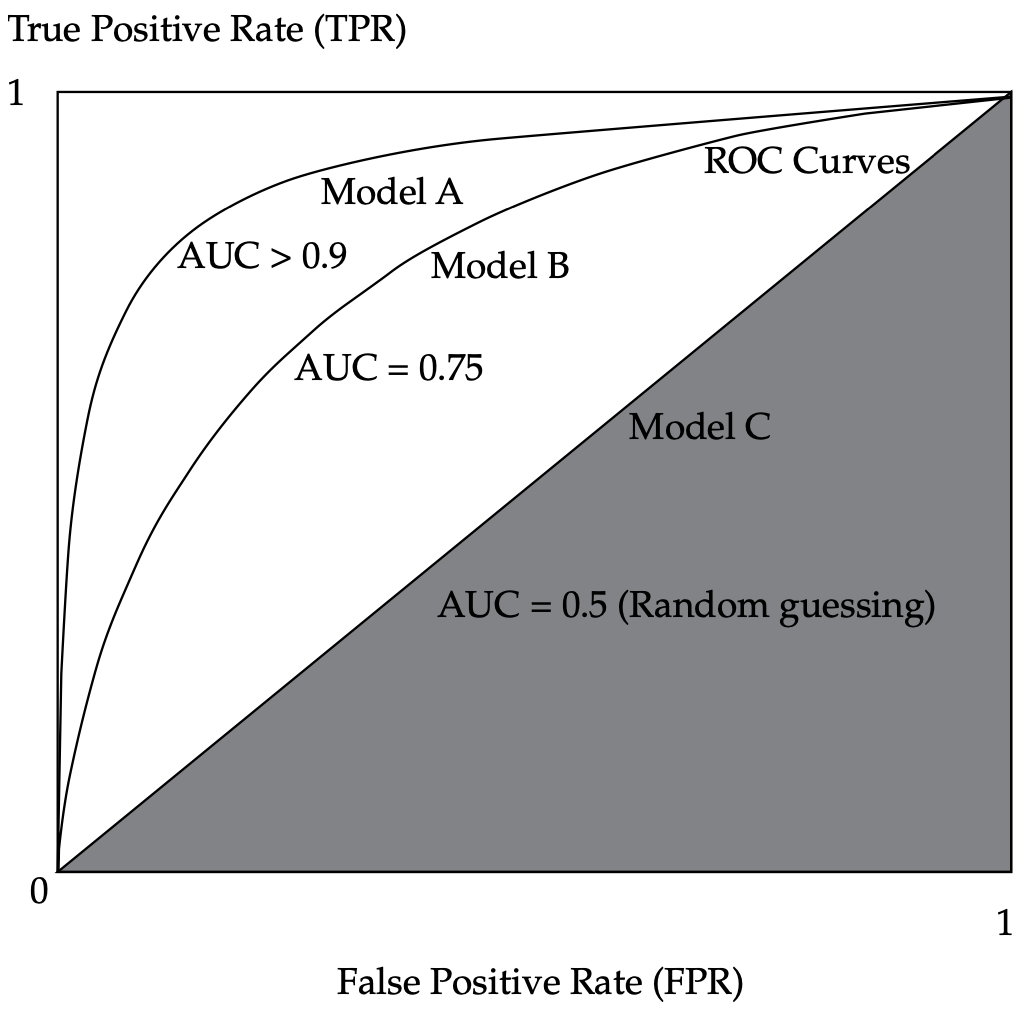
\includegraphics[scale=0.3]{/quant/aucroccurve}
\caption{ROC Curve}
\end{figure}

\begin{definition} \hlt{Root Mean Squared Error (RMSE)}\\
Useful for data predictions that are continuous, such as regression models.\\
The RMSE is a single metric summarising the prediction error in a sample.
$RMSE = \sqrt{\frac{1}{n} \sum\limits_{i=1}^n (\text{Predicted}_i - \text{Actual}_i)^2}$
\end{definition}

\begin{definition} \hlt{Grid Search}\\
Systematically train ML model using different combination of hyper-parameter values to determine combination of values that has best model performance.
\end{definition}

\begin{definition} \hlt{Regularisation}\\
Slight regularisation lightly penalises model complexity, thereby allowing most or all of the features to be included in the model and thus potentially enabling the model to memorise the data.\\
Large regularisation excessively penalises model complexity, thereby allowing too few of the features to be included in the model and causing the model to learn less from the data.\\
Optimum regularisation minimises both variance and bias errors in a balanced fashion. 
\end{definition}

\begin{figure}[H]
\centering
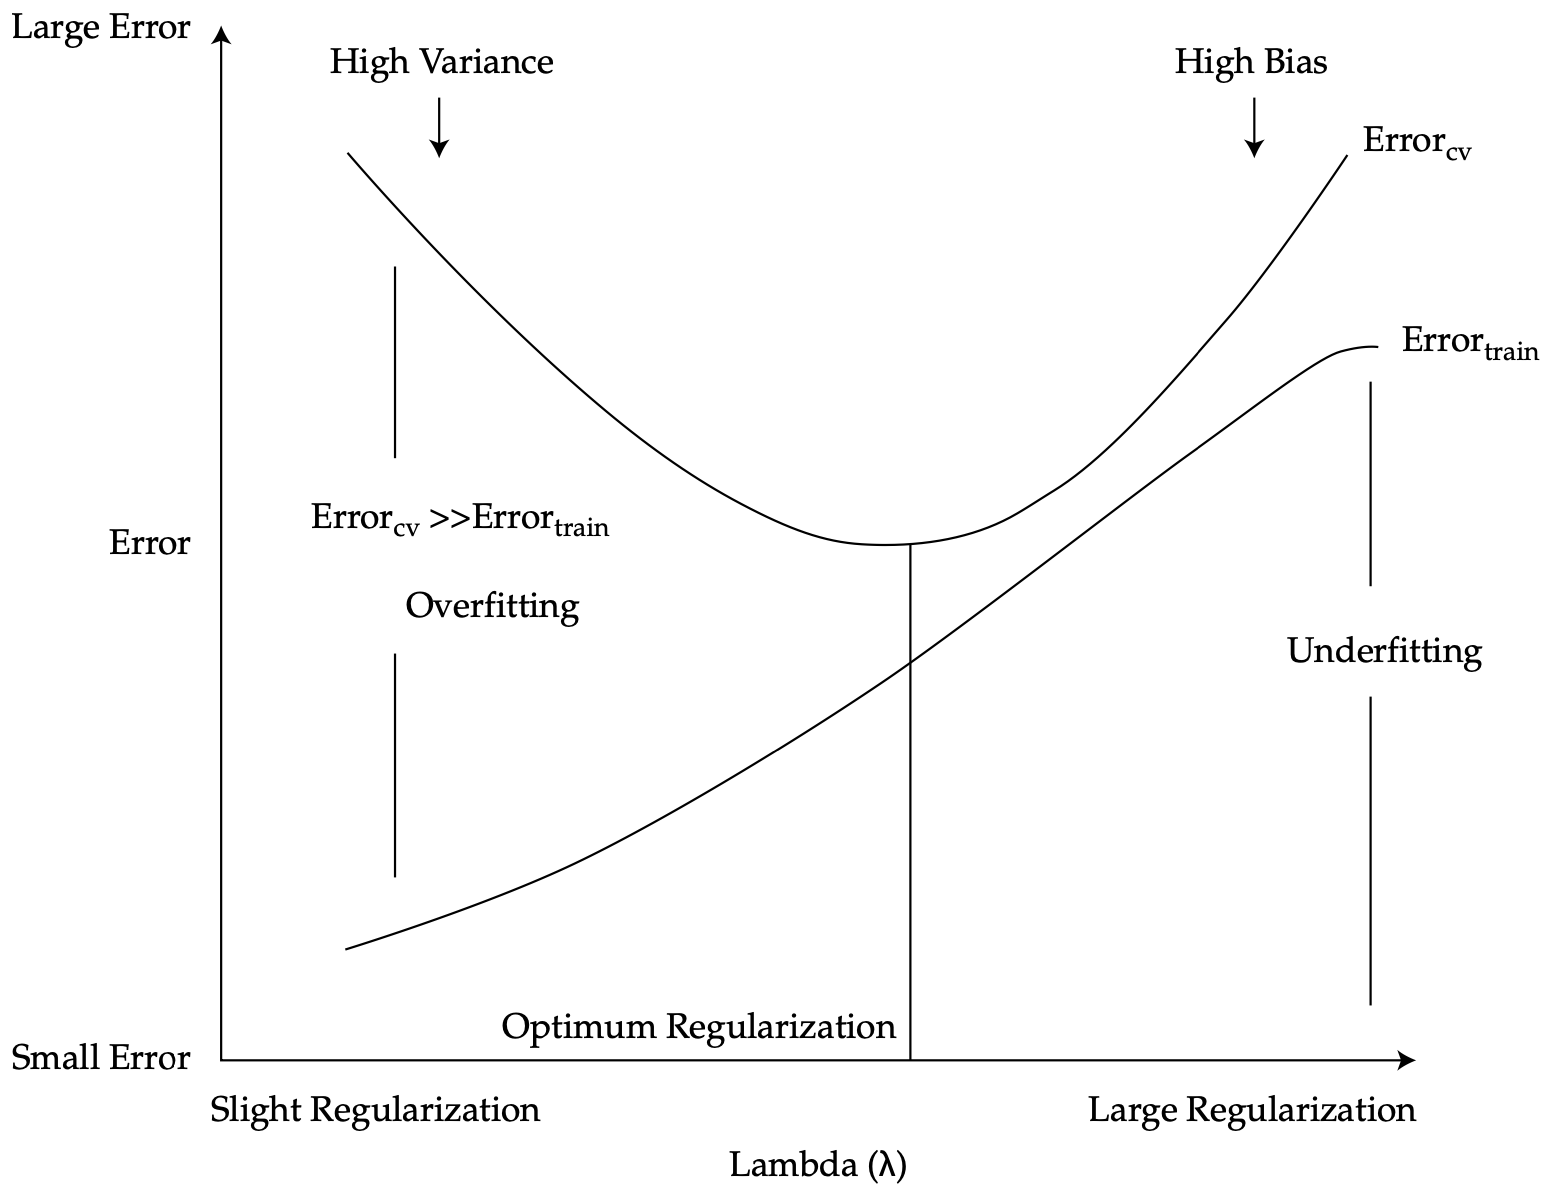
\includegraphics[scale=0.3]{/quant/hypparamfitcurve}
\caption{Fitting Curve for Regularisation Hyper-parameter $\lambda$}
\end{figure}

\begin{definition} \hlt{Ceiling Analysis}\\
Systematic process of evaluating different components in the pipeline of model building.\\
Determine which sub-model needs to be tuned to improve the overall accuracy of the larger model.
\end{definition}
